% Options for packages loaded elsewhere
\PassOptionsToPackage{unicode}{hyperref}
\PassOptionsToPackage{hyphens}{url}
\PassOptionsToPackage{dvipsnames,svgnames,x11names}{xcolor}
%
\documentclass[
  letterpaper,
  DIV=11,
  numbers=noendperiod]{scrreprt}

\usepackage{amsmath,amssymb}
\usepackage{iftex}
\ifPDFTeX
  \usepackage[T1]{fontenc}
  \usepackage[utf8]{inputenc}
  \usepackage{textcomp} % provide euro and other symbols
\else % if luatex or xetex
  \usepackage{unicode-math}
  \defaultfontfeatures{Scale=MatchLowercase}
  \defaultfontfeatures[\rmfamily]{Ligatures=TeX,Scale=1}
\fi
\usepackage{lmodern}
\ifPDFTeX\else  
    % xetex/luatex font selection
\fi
% Use upquote if available, for straight quotes in verbatim environments
\IfFileExists{upquote.sty}{\usepackage{upquote}}{}
\IfFileExists{microtype.sty}{% use microtype if available
  \usepackage[]{microtype}
  \UseMicrotypeSet[protrusion]{basicmath} % disable protrusion for tt fonts
}{}
\makeatletter
\@ifundefined{KOMAClassName}{% if non-KOMA class
  \IfFileExists{parskip.sty}{%
    \usepackage{parskip}
  }{% else
    \setlength{\parindent}{0pt}
    \setlength{\parskip}{6pt plus 2pt minus 1pt}}
}{% if KOMA class
  \KOMAoptions{parskip=half}}
\makeatother
\usepackage{xcolor}
\setlength{\emergencystretch}{3em} % prevent overfull lines
\setcounter{secnumdepth}{5}
% Make \paragraph and \subparagraph free-standing
\ifx\paragraph\undefined\else
  \let\oldparagraph\paragraph
  \renewcommand{\paragraph}[1]{\oldparagraph{#1}\mbox{}}
\fi
\ifx\subparagraph\undefined\else
  \let\oldsubparagraph\subparagraph
  \renewcommand{\subparagraph}[1]{\oldsubparagraph{#1}\mbox{}}
\fi

\usepackage{color}
\usepackage{fancyvrb}
\newcommand{\VerbBar}{|}
\newcommand{\VERB}{\Verb[commandchars=\\\{\}]}
\DefineVerbatimEnvironment{Highlighting}{Verbatim}{commandchars=\\\{\}}
% Add ',fontsize=\small' for more characters per line
\usepackage{framed}
\definecolor{shadecolor}{RGB}{241,243,245}
\newenvironment{Shaded}{\begin{snugshade}}{\end{snugshade}}
\newcommand{\AlertTok}[1]{\textcolor[rgb]{0.68,0.00,0.00}{#1}}
\newcommand{\AnnotationTok}[1]{\textcolor[rgb]{0.37,0.37,0.37}{#1}}
\newcommand{\AttributeTok}[1]{\textcolor[rgb]{0.40,0.45,0.13}{#1}}
\newcommand{\BaseNTok}[1]{\textcolor[rgb]{0.68,0.00,0.00}{#1}}
\newcommand{\BuiltInTok}[1]{\textcolor[rgb]{0.00,0.23,0.31}{#1}}
\newcommand{\CharTok}[1]{\textcolor[rgb]{0.13,0.47,0.30}{#1}}
\newcommand{\CommentTok}[1]{\textcolor[rgb]{0.37,0.37,0.37}{#1}}
\newcommand{\CommentVarTok}[1]{\textcolor[rgb]{0.37,0.37,0.37}{\textit{#1}}}
\newcommand{\ConstantTok}[1]{\textcolor[rgb]{0.56,0.35,0.01}{#1}}
\newcommand{\ControlFlowTok}[1]{\textcolor[rgb]{0.00,0.23,0.31}{#1}}
\newcommand{\DataTypeTok}[1]{\textcolor[rgb]{0.68,0.00,0.00}{#1}}
\newcommand{\DecValTok}[1]{\textcolor[rgb]{0.68,0.00,0.00}{#1}}
\newcommand{\DocumentationTok}[1]{\textcolor[rgb]{0.37,0.37,0.37}{\textit{#1}}}
\newcommand{\ErrorTok}[1]{\textcolor[rgb]{0.68,0.00,0.00}{#1}}
\newcommand{\ExtensionTok}[1]{\textcolor[rgb]{0.00,0.23,0.31}{#1}}
\newcommand{\FloatTok}[1]{\textcolor[rgb]{0.68,0.00,0.00}{#1}}
\newcommand{\FunctionTok}[1]{\textcolor[rgb]{0.28,0.35,0.67}{#1}}
\newcommand{\ImportTok}[1]{\textcolor[rgb]{0.00,0.46,0.62}{#1}}
\newcommand{\InformationTok}[1]{\textcolor[rgb]{0.37,0.37,0.37}{#1}}
\newcommand{\KeywordTok}[1]{\textcolor[rgb]{0.00,0.23,0.31}{#1}}
\newcommand{\NormalTok}[1]{\textcolor[rgb]{0.00,0.23,0.31}{#1}}
\newcommand{\OperatorTok}[1]{\textcolor[rgb]{0.37,0.37,0.37}{#1}}
\newcommand{\OtherTok}[1]{\textcolor[rgb]{0.00,0.23,0.31}{#1}}
\newcommand{\PreprocessorTok}[1]{\textcolor[rgb]{0.68,0.00,0.00}{#1}}
\newcommand{\RegionMarkerTok}[1]{\textcolor[rgb]{0.00,0.23,0.31}{#1}}
\newcommand{\SpecialCharTok}[1]{\textcolor[rgb]{0.37,0.37,0.37}{#1}}
\newcommand{\SpecialStringTok}[1]{\textcolor[rgb]{0.13,0.47,0.30}{#1}}
\newcommand{\StringTok}[1]{\textcolor[rgb]{0.13,0.47,0.30}{#1}}
\newcommand{\VariableTok}[1]{\textcolor[rgb]{0.07,0.07,0.07}{#1}}
\newcommand{\VerbatimStringTok}[1]{\textcolor[rgb]{0.13,0.47,0.30}{#1}}
\newcommand{\WarningTok}[1]{\textcolor[rgb]{0.37,0.37,0.37}{\textit{#1}}}

\providecommand{\tightlist}{%
  \setlength{\itemsep}{0pt}\setlength{\parskip}{0pt}}\usepackage{longtable,booktabs,array}
\usepackage{calc} % for calculating minipage widths
% Correct order of tables after \paragraph or \subparagraph
\usepackage{etoolbox}
\makeatletter
\patchcmd\longtable{\par}{\if@noskipsec\mbox{}\fi\par}{}{}
\makeatother
% Allow footnotes in longtable head/foot
\IfFileExists{footnotehyper.sty}{\usepackage{footnotehyper}}{\usepackage{footnote}}
\makesavenoteenv{longtable}
\usepackage{graphicx}
\makeatletter
\def\maxwidth{\ifdim\Gin@nat@width>\linewidth\linewidth\else\Gin@nat@width\fi}
\def\maxheight{\ifdim\Gin@nat@height>\textheight\textheight\else\Gin@nat@height\fi}
\makeatother
% Scale images if necessary, so that they will not overflow the page
% margins by default, and it is still possible to overwrite the defaults
% using explicit options in \includegraphics[width, height, ...]{}
\setkeys{Gin}{width=\maxwidth,height=\maxheight,keepaspectratio}
% Set default figure placement to htbp
\makeatletter
\def\fps@figure{htbp}
\makeatother
\newlength{\cslhangindent}
\setlength{\cslhangindent}{1.5em}
\newlength{\csllabelwidth}
\setlength{\csllabelwidth}{3em}
\newlength{\cslentryspacingunit} % times entry-spacing
\setlength{\cslentryspacingunit}{\parskip}
\newenvironment{CSLReferences}[2] % #1 hanging-ident, #2 entry spacing
 {% don't indent paragraphs
  \setlength{\parindent}{0pt}
  % turn on hanging indent if param 1 is 1
  \ifodd #1
  \let\oldpar\par
  \def\par{\hangindent=\cslhangindent\oldpar}
  \fi
  % set entry spacing
  \setlength{\parskip}{#2\cslentryspacingunit}
 }%
 {}
\usepackage{calc}
\newcommand{\CSLBlock}[1]{#1\hfill\break}
\newcommand{\CSLLeftMargin}[1]{\parbox[t]{\csllabelwidth}{#1}}
\newcommand{\CSLRightInline}[1]{\parbox[t]{\linewidth - \csllabelwidth}{#1}\break}
\newcommand{\CSLIndent}[1]{\hspace{\cslhangindent}#1}

\KOMAoption{captions}{tableheading}
\makeatletter
\makeatother
\makeatletter
\@ifpackageloaded{bookmark}{}{\usepackage{bookmark}}
\makeatother
\makeatletter
\@ifpackageloaded{caption}{}{\usepackage{caption}}
\AtBeginDocument{%
\ifdefined\contentsname
  \renewcommand*\contentsname{Table of contents}
\else
  \newcommand\contentsname{Table of contents}
\fi
\ifdefined\listfigurename
  \renewcommand*\listfigurename{List of Figures}
\else
  \newcommand\listfigurename{List of Figures}
\fi
\ifdefined\listtablename
  \renewcommand*\listtablename{List of Tables}
\else
  \newcommand\listtablename{List of Tables}
\fi
\ifdefined\figurename
  \renewcommand*\figurename{Figure}
\else
  \newcommand\figurename{Figure}
\fi
\ifdefined\tablename
  \renewcommand*\tablename{Table}
\else
  \newcommand\tablename{Table}
\fi
}
\@ifpackageloaded{float}{}{\usepackage{float}}
\floatstyle{ruled}
\@ifundefined{c@chapter}{\newfloat{codelisting}{h}{lop}}{\newfloat{codelisting}{h}{lop}[chapter]}
\floatname{codelisting}{Listing}
\newcommand*\listoflistings{\listof{codelisting}{List of Listings}}
\makeatother
\makeatletter
\@ifpackageloaded{caption}{}{\usepackage{caption}}
\@ifpackageloaded{subcaption}{}{\usepackage{subcaption}}
\makeatother
\makeatletter
\@ifpackageloaded{tcolorbox}{}{\usepackage[skins,breakable]{tcolorbox}}
\makeatother
\makeatletter
\@ifundefined{shadecolor}{\definecolor{shadecolor}{rgb}{.97, .97, .97}}
\makeatother
\makeatletter
\makeatother
\makeatletter
\makeatother
\ifLuaTeX
  \usepackage{selnolig}  % disable illegal ligatures
\fi
\IfFileExists{bookmark.sty}{\usepackage{bookmark}}{\usepackage{hyperref}}
\IfFileExists{xurl.sty}{\usepackage{xurl}}{} % add URL line breaks if available
\urlstyle{same} % disable monospaced font for URLs
\hypersetup{
  pdftitle={Disease Surveillance},
  colorlinks=true,
  linkcolor={blue},
  filecolor={Maroon},
  citecolor={Blue},
  urlcolor={Blue},
  pdfcreator={LaTeX via pandoc}}

\title{Disease Surveillance}
\author{}
\date{}

\begin{document}
\maketitle
\ifdefined\Shaded\renewenvironment{Shaded}{\begin{tcolorbox}[sharp corners, interior hidden, breakable, frame hidden, boxrule=0pt, enhanced, borderline west={3pt}{0pt}{shadecolor}]}{\end{tcolorbox}}\fi

\renewcommand*\contentsname{Table of contents}
{
\hypersetup{linkcolor=}
\setcounter{tocdepth}{2}
\tableofcontents
}
\bookmarksetup{startatroot}

\hypertarget{welcome-to-the-disease-surveillance-project}{%
\chapter*{Welcome to the disease surveillance
project!}\label{welcome-to-the-disease-surveillance-project}}
\addcontentsline{toc}{chapter}{Welcome to the disease surveillance
project!}

\markboth{Welcome to the disease surveillance project!}{Welcome to the
disease surveillance project!}

We provide tools to national health organizations that allow them to
make the best use of their data to improve the health and quality of
life of their populations. Our work primarily focus on surveillance of
climate-sensitive diseases such as dengue in Brazil and malaria in
Africa.

We develop innovative statistical and machine learning methods to help
understand the geographical spread of diseases and forecast future
cases. Our methods leverage multiple datasets from various sources,
including temperature, precipitation, and socio-economic factors.
Additionally, we use digital data sources to help determine disease
levels in real-time.

Our project aims to be a valuable resource for decision-makers and the
general public seeking information on disease levels in various
countries. We also provide researchers useful methods and software tools
that they can utilize in their efforts to monitor diseases and guide
decision-making in their own surveillance applications.

\begin{figure}

{\centering \includegraphics[width=1\textwidth,height=\textheight]{img/stripes1850-2022-MO.png}

}

\caption{\label{fig-stripes}\href{https://showyourstripes.info/}{\#ShowYourStripes}.}

\end{figure}

\bookmarksetup{startatroot}

\hypertarget{people}{%
\chapter*{People}\label{people}}
\addcontentsline{toc}{chapter}{People}

\markboth{People}{People}

The disease surveillance project is led by Paula Moraga, Assistant
Professor of Statistics and PI of the GeoHealth research group at King
Abdullah University of Science and Technology (KAUST). Funding for this
work is provided by the \href{https://letten.foundation/}{Letten
Foundation}.

The project's success is reliant on the cooperation of a number of
collaborators and organizations worldwide. The team members listed below
work on the development of statistical and machine learning methods for
disease surveillance, and the translation of findings into actionable
initiatives that improve health and wellbeing for all.

Paula Moraga KAUST

Xiang Chen KAUST

Yang Xiao KAUST

Guilherme Soares University of São Paulo

Rafael Izbicki Federal University of São Carlos

Leo Bastos Fiocruz

Mario Gómez University of Costa Rica

Luis Barboza University of Costa Rica

\includegraphics{01-people_files/figure-pdf/unnamed-chunk-1-1.pdf}

\part{Data}

\hypertarget{data-1}{%
\chapter{Data}\label{data-1}}

\hypertarget{official-disease-data}{%
\section{Official disease data}\label{official-disease-data}}

Ministries and departments of health

\begin{itemize}
\tightlist
\item
  Cases (number of individual cases reported)
\end{itemize}

\hypertarget{digital-data-sources}{%
\section{Digital data sources}\label{digital-data-sources}}

Search query data, social media data

\begin{itemize}
\tightlist
\item
  Google trends data (index from 0 to 100)
\end{itemize}

\hypertarget{population}{%
\section{Population}\label{population}}

The \href{https://wopr.worldpop.org/}{WorldPop Open Population
Repository} provides access to gridded population estimates.

\hypertarget{climatic-and-environmental-data}{%
\section{Climatic and environmental
data}\label{climatic-and-environmental-data}}

For each of the covariates, review on how it affects
dengue/malaria/other infectious disease and references.

\begin{itemize}
\tightlist
\item
  Temperature
\item
  Precipitation
\item
  Humidity
\item
  El Niño/Southern Oscillation (ENSO) index
\item
  Historical and future data
\end{itemize}

\href{https://cds.climate.copernicus.eu/}{Copernicus climate data store}

The R Package \href{https://github.com/ErikKusch/KrigR}{KrigR} allows us
to download, preprocess, and downscale data from the European Centre for
Medium-range Weather Forecasts ReAnalysis 5 (ERA5) family provided by
the European Centre for Medium‐Range Weather Forecasts (ECMWF). The
package interfaces with the
\href{https://cds.climate.copernicus.eu/\#!/home}{Climate Data Store
(CDS)} hosted by the Copernicus
\href{https://cds.climate.copernicus.eu/about-c3s}{Climate Change
Service (C3S)} for retrieval of climate data. To use it, we need to
create a CDS \href{https://cds.climate.copernicus.eu/api-how-to}{API
Key}.

The R package \href{https://agrdatasci.github.io/ag5Tools/}{ag5Tools}
allows us to download and extract data from the ``Agrometeorological
indicators from 1979 to present and a spatial resolution of
0.1\(^o \times\) 0.1\(^o\) (approximately 11 km \(\times\) 11 km at the
equator) derived from reanalysis'' dataset
(\href{https://cds.climate.copernicus.eu/cdsapp\#!/dataset/10.24381/cds.6c68c9bb?tab=overview}{AgERA5}).

\hypertarget{environment}{%
\section{Environment}\label{environment}}

\hypertarget{socio-economic}{%
\section{Socio-economic}\label{socio-economic}}

\hypertarget{covariates-repositories}{%
\section{Covariates repositories}\label{covariates-repositories}}

\begin{longtable}[]{@{}
  >{\raggedright\arraybackslash}p{(\columnwidth - 10\tabcolsep) * \real{0.1316}}
  >{\raggedright\arraybackslash}p{(\columnwidth - 10\tabcolsep) * \real{0.2632}}
  >{\raggedright\arraybackslash}p{(\columnwidth - 10\tabcolsep) * \real{0.2763}}
  >{\raggedright\arraybackslash}p{(\columnwidth - 10\tabcolsep) * \real{0.1053}}
  >{\raggedright\arraybackslash}p{(\columnwidth - 10\tabcolsep) * \real{0.1053}}
  >{\raggedright\arraybackslash}p{(\columnwidth - 10\tabcolsep) * \real{0.1184}}@{}}
\toprule\noalign{}
\endhead
\bottomrule\noalign{}
\endlastfoot
Variable & Spatial resolution & Temporal resolution & Time period &
Source & Package \\
Temperature & & & 1979-present and future? & & \\
Precipitation & & & & & \\
Humidity & & & & & \\
El Niño/Southern Oscillation (ENSO) & & & & & \\
\end{longtable}

\part{Surveillance methods}

\hypertarget{disease-mapping}{%
\chapter{Disease mapping}\label{disease-mapping}}

\hypertarget{nowcasting}{%
\chapter{Nowcasting}\label{nowcasting}}

\includegraphics[width=6.25in,height=\textheight]{img/nowcastingleobastos.png}

From Bastos et al. (2019)

\begin{itemize}
\tightlist
\item
  Less than 50\% cases are reported in one week
\item
  Less than 75\% cases are reported in four weeks
\item
  Less than 90\% cases are reported in nine weeks
\end{itemize}

\hypertarget{forecasting}{%
\chapter{Forecasting}\label{forecasting}}

\part{Communication}

\hypertarget{visualization}{%
\chapter{Visualization}\label{visualization}}

\part{Dengue in Brazil}

\hypertarget{dengue}{%
\chapter{Dengue}\label{dengue}}

Dengue is a viral infection that spreads to people through the bite of
an infected \emph{Aedes} species (\emph{Aedes aegypti} or \emph{Aedes
albopictus}) mosquito. About half of the global population is currently
at risk of contracting dengue fever, with an estimated 100 to 400
million infections occurring annually. Dengue is prevalent in tropical
and subtropical regions worldwide, primarily in urban and semi-urban
areas.

\begin{figure}

{\centering \includegraphics[width=11.33in,height=\textheight]{img/dengueincidence.png}

}

\caption{\label{fig-dengueincidence}\href{https://ourworldindata.org/grapher/dengue-incidence}{Dengue
incidence}.}

\end{figure}

Although many infections of the dengue virus (DENV) do not show symptoms
or only result in mild flu-like illness, some cases can be severe and
potentially fatal. Dengue fever does not have a specific treatment.
Early detection and timely access to proper medical care significantly
reduce the fatality rates associated with severe cases. Preventing and
controlling dengue transmission relies on managing the the mosquitoes
that act as vectors.

\begin{figure}

{\centering \includegraphics[width=0.49\textwidth,height=\textheight]{img/aedesaegypti.jpg}

}

\caption{\label{fig-aedesaegypti}\href{https://en.wikipedia.org/wiki/Aedes_aegypti\#/media/File:Aedes_aegypti_CDC-Gathany.jpg}{Aedes
Aegypti}}

\end{figure}

\begin{figure}

{\centering \includegraphics[width=0.49\textwidth,height=\textheight]{img/vectorcontrolefforts.jpg}

}

\caption{\label{fig-vectorcontrolefforts}\href{https://en.wikipedia.org/wiki/Dengue_fever\#/media/File:Equipes_usam_t\%C3\%A9cnicas_de_combate_\%C3\%A0_dengue_em_Bras\%C3\%ADlia.jpg}{Vector
control efforts}.}

\end{figure}

\hypertarget{dengue-tracker}{%
\chapter{Dengue tracker}\label{dengue-tracker}}

Dengue data from surveillance systems is crucial for prevention and
control. Unfortunately, this data is often delayed, preventing timely
decision-making and resource allocation. In
\href{https://diseasesurveillance.github.io/dengue-tracker/index.html}{Dengue-tracker},
we provide weekly updates on the number of official dengue cases per
municipality in Brazil. Additionally, we present corrected case counts
incorporating information from Google trends. We believe these reports
will assist policymakers and the general public in understanding dengue
levels and guide their decisions.

\begin{quote}
\href{https://diseasesurveillance.github.io/dengue-tracker/index.html}{\textbf{Click
here to access Dengue-tracker}}
\end{quote}

\begin{figure}

{\centering \includegraphics[width=1\textwidth,height=\textheight]{img/denguetracker.png}

}

\caption{\label{fig-denguetracker}\href{https://diseasesurveillance.github.io/dengue-tracker/index.html}{Dengue-tracker}}

\end{figure}

\hypertarget{ews}{%
\chapter{EWS}\label{ews}}

We are developing a disease surveillance system to forecast the future
number of cases and the early detection of disease outbreaks. We are
validating the system using dengue data from Brazil.

\hypertarget{system-components}{%
\subsection*{System components}\label{system-components}}
\addcontentsline{toc}{subsection}{System components}

\begin{itemize}
\tightlist
\item
  Data retrieval of official dengue data, search query data, population,
  climate and environmental covariates (download, clean and format data
  for analysis and visualization)
\item
  Nowcasting methods using digital, environmental and climate data. Data
  include temperature, precipitation, and Google trends using specific
  keywords related to dengue)
\item
  Forecasting methods using environmental and climate data (and ensemble
  of several methods)
\item
  Methods for monitoring dengue in one municipality, and extension to
  models that borrow information from neighboring regions
\item
  Methods performance by quantifying how well the methods predict future
  number of cases weeks or months in advance
\item
  Software system to be used to monitor dengue in Brazil, and adaptable
  to other diseases and countries
\end{itemize}

\hypertarget{forecasting-methods}{%
\subsection*{Forecasting methods}\label{forecasting-methods}}
\addcontentsline{toc}{subsection}{Forecasting methods}

\includegraphics[width=6.25in,height=\textheight]{img/denguebrazil-forecasts-movewindow.png}

\includegraphics[width=6.25in,height=\textheight]{img/denguebrazil-realvsforecasts.jpg}

\hypertarget{data-2}{%
\chapter{Data}\label{data-2}}

\hypertarget{map-of-brazilian-municipalities}{%
\section{Map of Brazilian
municipalities}\label{map-of-brazilian-municipalities}}

R package
\href{https://cran.r-project.org/web/packages/geobr/vignettes/intro_to_geobr.html}{\textbf{geobr}}

\begin{Shaded}
\begin{Highlighting}[]
\FunctionTok{library}\NormalTok{(geobr)}
\FunctionTok{library}\NormalTok{(ggplot2)}

\NormalTok{map }\OtherTok{\textless{}{-}} \FunctionTok{read\_state}\NormalTok{(}\AttributeTok{year =} \DecValTok{2020}\NormalTok{, }\AttributeTok{showProgress =} \ConstantTok{FALSE}\NormalTok{)}
\CommentTok{\# length(unique(map$code\_state)) \# number of states: 27}
\FunctionTok{ggplot}\NormalTok{(map) }\SpecialCharTok{+} \FunctionTok{geom\_sf}\NormalTok{() }\SpecialCharTok{+} \FunctionTok{labs}\NormalTok{(}\AttributeTok{title =} \StringTok{"States"}\NormalTok{)}
\end{Highlighting}
\end{Shaded}

\begin{figure}[H]

{\centering \includegraphics{59-denguebrazil-data_files/figure-pdf/unnamed-chunk-1-1.pdf}

}

\end{figure}

\begin{Shaded}
\begin{Highlighting}[]
\NormalTok{map }\OtherTok{\textless{}{-}} \FunctionTok{read\_micro\_region}\NormalTok{(}\AttributeTok{year =} \DecValTok{2020}\NormalTok{, }\AttributeTok{showProgress =} \ConstantTok{FALSE}\NormalTok{)}
\CommentTok{\# length(unique(map$code\_micro)) \# number of microregions: 558}
\FunctionTok{ggplot}\NormalTok{(map) }\SpecialCharTok{+} \FunctionTok{geom\_sf}\NormalTok{() }\SpecialCharTok{+} \FunctionTok{labs}\NormalTok{(}\AttributeTok{title =} \StringTok{"Microregions"}\NormalTok{)}
\end{Highlighting}
\end{Shaded}

\begin{figure}[H]

{\centering 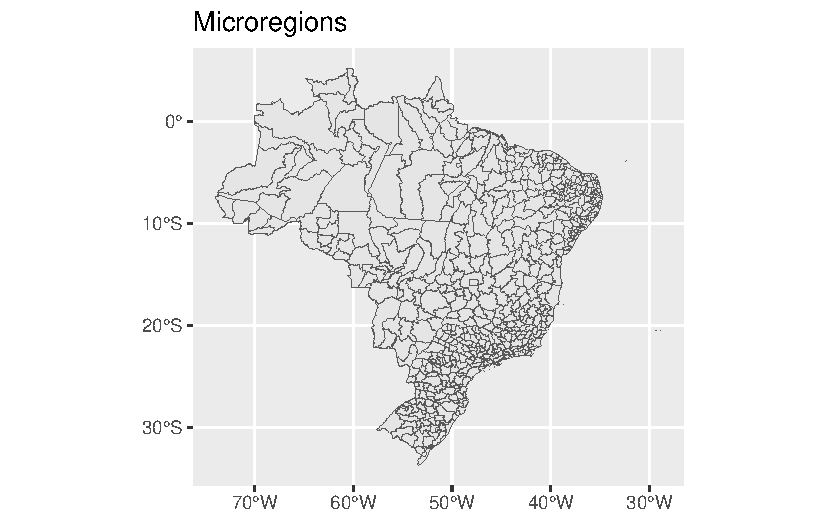
\includegraphics{59-denguebrazil-data_files/figure-pdf/unnamed-chunk-1-2.pdf}

}

\end{figure}

\begin{Shaded}
\begin{Highlighting}[]
\NormalTok{map }\OtherTok{\textless{}{-}} \FunctionTok{read\_municipality}\NormalTok{(}\AttributeTok{year =} \DecValTok{2020}\NormalTok{, }\AttributeTok{showProgress =} \ConstantTok{FALSE}\NormalTok{)}
\CommentTok{\# length(unique(map$code\_muni)) \# number of municipalities: 5570}
\FunctionTok{ggplot}\NormalTok{(map) }\SpecialCharTok{+} \FunctionTok{geom\_sf}\NormalTok{() }\SpecialCharTok{+} \FunctionTok{labs}\NormalTok{(}\AttributeTok{title =} \StringTok{"Municipalities"}\NormalTok{)}
\end{Highlighting}
\end{Shaded}

\hypertarget{dengue-data}{%
\section{Dengue data}\label{dengue-data}}

\href{https://info.dengue.mat.br/}{InfoDengue}

\href{https://info.dengue.mat.br/services/tutorial/R}{InfoDengue API}

Dengue cases, nowcasts, temperature and humidity by city level and
epidemiological week

\begin{verbatim}
url <- "https://info.dengue.mat.br/api/alertcity?"
geocode <- 3304557
disease <- "dengue"
format <- "csv"
ew_start <- 1
ew_end <- 52
ey_start <- 2021
ey_end <- 2021

cons1 <- paste0(url,"geocode=",geocode,"&disease=",disease,"&format=",format,"&ew_start=",ew_start,"&ew_end=",ew_end,"&ey_start=",ey_start,"&ey_end=",ey_end)


library(tidyverse)
d <- read_csv(cons1, show_col_types=FALSE) %>% arrange(data_iniSE)
glimpse(d)
ggplot(d, aes(SE, casos)) + geom_line()
\end{verbatim}

\includegraphics[width=6.25in,height=\textheight]{img/denguebrazil-incidence.png}

Dengue incidence rate (cases per 100 000 residents per month) for ten
Brazilian states (São Paulo and Minas Gerais from the southeast, Rio
Grande do Sul and Santa Catarina from the south, Mato Grosso do Sul and
Goias from the midwest, Ceará and Bahia from the northeast, Pará and
Amazonas from the north). It is clear that the incidence rate is
influenced by geographical and environmental factors, as described in
Lowe et al. (2021)

\hypertarget{google-trends-data}{%
\section{Google trends data}\label{google-trends-data}}

\includegraphics[width=1\textwidth,height=\textheight]{img/denguebrazil-googletrends.png}

Google trends dengue data. Values in a range of 0 to 100, where 100
represents the maximal value. Each data point is divided by the total
searches of the geography and time range it represents to compare
relative popularity. Otherwise, places with the most search volume would
always be ranked highest

\begin{figure}

{\centering \includegraphics[width=0.6\textwidth,height=\textheight]{img/denguebrazil-corrofficialgoogle.png}

}

\end{figure}

\hypertarget{population-1}{%
\section{Population}\label{population-1}}

\hypertarget{climate}{%
\section{Climate}\label{climate}}

\begin{itemize}
\tightlist
\item
  Temperature
\item
  Precipitation
\item
  Humidity
\item
  El Niño/Southern Oscillation (ENSO) index
\item
  Historical and future data
\end{itemize}

\hypertarget{environment-1}{%
\section{Environment}\label{environment-1}}

\hypertarget{socio-economic-1}{%
\section{Socio-economic}\label{socio-economic-1}}

\part{Training}

\hypertarget{resources}{%
\chapter{Resources}\label{resources}}

\hypertarget{books-on-spatial-data-analysis-and-visualization}{%
\section{Books on spatial data analysis and
visualization}\label{books-on-spatial-data-analysis-and-visualization}}

Spatial Statistics for Data Science: Theory and Practice with R Moraga.
Chapman \& Hall/CRC Data Science Series (2023)

Geospatial Health Data: Modeling and Visualization with R-INLA and Shiny
Moraga. Chapman \& Hall/CRC Biostatistics Series (2019)

\hypertarget{downloading-climate-and-environmental-data}{%
\section{Downloading climate and environmental
data}\label{downloading-climate-and-environmental-data}}

\href{https://github.com/ErikKusch/KrigR}{KrigR: an R package to
download data from ERA5 from ECMWF}

\href{https://rspatialdata.github.io/index.html}{rspatialdata tutorials}

\hypertarget{interactive-visualizations}{%
\section{Interactive Visualizations}\label{interactive-visualizations}}

\href{https://www.htmlwidgets.org/}{htmlwidgets for R}

\href{https://rstudio.github.io/leaflet/}{leaflet}

\href{https://dreamrs.github.io/apexcharter/}{apexcharter}

\hypertarget{building-shiny-web-applications}{%
\section{Building Shiny web
applications}\label{building-shiny-web-applications}}

\href{https://shiny.posit.co/}{Shiny}

\bookmarksetup{startatroot}

\hypertarget{references}{%
\chapter*{References}\label{references}}
\addcontentsline{toc}{chapter}{References}

\markboth{References}{References}

\hypertarget{refs}{}
\begin{CSLReferences}{1}{0}
\leavevmode\vadjust pre{\hypertarget{ref-bastosetal19}{}}%
Bastos, Leonardo S., Theodoros Economou, Marcelo F. C. Gomes, Daniel A.
M. Villela, Flavio C Coelho, Oswaldo G. Cruz, Oliver Stoner, Trevor
Bailey, and Claudia T. Codeço. 2019. {``{A modelling approach for
correcting reporting delays in disease surveillance data}.''}
\emph{{Statistics in Medicine}}. \url{https://doi.org/10.1002/sim.8303}.

\leavevmode\vadjust pre{\hypertarget{ref-loweetal21}{}}%
Lowe, Rachel, Sophie A Lee, Kathleen M O'Reilly, Oliver J Brady,
Leonardo Bastos, Gabriel Carrasco-Escobar, Rafael de Castro Catão, et
al. 2021. {``{Combined effects of hydrometeorological hazards and
urbanisation on dengue risk in Brazil: a spatiotemporal modelling
study}.''} \emph{{The Lancet Planetary Health}}.
\url{https://doi.org/10.1016/S2542-5196(20)30292-8}.

\end{CSLReferences}



\end{document}
